\documentclass[a4paper,10pt]{article}

\usepackage{url}

\usepackage{geometry}
\geometry{
paperwidth = 200mm,
paperheight = 150mm,
 %a4paper,
 %total={200mm,240mm},
 left=15mm,
 right=10mm,
 top=10mm,
bottom=10mm
}

%\usepackage[a4,frame,center]{crop}

\usepackage{kotex}  % to use korean text


% following three lines select font size similar to 'Times New Roman'. Actually ptm, phv and pcr stands for adobe times, adobe helvetica and adobe courier. ptm changes default CM Roman to Times Roman.
%\renewcommand{\sfdefault}{phv}
%\renewcommand{\rmdefault}{ptm}
%\renewcommand{\ttdefault}{pcr}
% alternatively, this can also be achieved by simply using a package 
\usepackage{mathptmx}  

\newcommand{\bitl}[1]{\textbf{\textit{#1}}} % new command to bold and italicize


\usepackage[linewidth=2pt]{mdframed} % to draw box around text

\setlength\parindent{0pt}  % set the indent as 0

\pagenumbering{gobble}  % to hide page numbers

\usepackage{verbatim}  % for multiline comment

\usepackage{setspace}  % to change line space locally

\usepackage[dvipsnames, table]{xcolor}  % to use colors

\definecolor{codepurple}{rgb}{0.58,0,0.82}
\definecolor{backcolour}{rgb}{0.95,0.95,0.92}
\definecolor{MyOwnColor}{RGB}{219, 48, 122}

\newcommand{\codize}[1]{\colorbox{BurntOrange}{\textcolor{MyOwnColor}{#1}}}

\usepackage{listings} % for source code display
\lstset
{
    language=[LaTeX]TeX,
    breaklines=true,
    basicstyle=\tt\scriptsize,
    keywordstyle=\color{blue},
    stringstyle=\color{mauve},
    commentstyle=\color{codepurple},
    backgroundcolor=\color{backcolour}, 
    identifierstyle=\color{magenta},
}


% following lines make it possible to show latex source code with colors
% usage: \lstinline[style=A]|\LaTeX|  is fun.
\usepackage{showexpl}
\lstdefinestyle{Common}
{   
    language={[LaTeX]TeX},
    numbers=left,
    numbersep=1em,
    %numberstyle=\tiny\noaccsupp,
    frame=single,
    framesep=\fboxsep,
    framerule=\fboxrule,
    rulecolor=\color{red},
    xleftmargin=\dimexpr\fboxsep+\fboxrule,
    xrightmargin=\dimexpr\fboxsep+\fboxrule,
    breaklines=true,
    breakindent=0pt,
    tabsize=2,
    columns=flexible,
    includerangemarker=false,
    rangeprefix=//\ ,
}
\lstdefinestyle{A}
{
    style=Common,
    backgroundcolor=\color{MyOwnColor},
    basicstyle=\scriptsize\ttfamily,
    keywordstyle=\color{MyOwnColor}\bf,
    identifierstyle=\color{MyOwnColor},
    stringstyle=\color{red},
    commentstyle=\color{green}
}



\usepackage{trackchanges}
\renewcommand{\initialsOne}{FS}
\renewcommand{\initialsTwo}{PS}

\newenvironment{tightcenter}{%
  \setlength\topsep{0pt}
  \setlength\parskip{0pt}
  \begin{center}
}{%
  \end{center}
  \vspace{20pt}
}

\renewcommand{\baselinestretch}{1.5} % line spacing

\newcommand{\latex}{\LaTeX\xspace}
\newcommand{\tex}{\TeX\xspace}

\usepackage[super]{nth}  % to write 1st, 2nd etc.

\usepackage{amsmath, amsfonts, amsthm} % for mathematics

% for figures
\usepackage{graphicx}
\usepackage{wrapfig}
\usepackage{float}


\usepackage{lipsum}  % generate non-sense text

\newcommand{\nopar}{{\parfillskip=0pt \par}}

\usepackage{tikz}

\usepackage{multirow}  % combining rows in table


\usepackage{longtable}


\usepackage[colorlinks]{hyperref}
\hypersetup{%
  colorlinks = true,
  linkcolor  = black,
  citecolor= blue
}

\usepackage[square]{natbib}

% for table generation from csv files
\usepackage{booktabs} % For \toprule, \midrule and \bottomrule
\usepackage{siunitx} % Formats the units and values
\usepackage{pgfplotstable} % Generates table from .csv
\sisetup{
  round-mode          = places, % Rounds numbers
  round-precision     = 2, % to 2 places
}





















\begin{document}
\begin{comment}
\title{Demonstration of trackchanges.sty}
\author{Felix Salfner}

\maketitle

\begin{abstract} \noindent The intention of this text is to demonstrate the use of \texttt{trackchanges.sty}. The package defines five editing commands:
\begin{itemize}
  \item \begin{verbatim}\note[initials]{note text}\end{verbatim}
  \item \begin{verbatim}\annote[initials]{note text}\end{verbatim}
  \item \begin{verbatim}\add[initials]{additional text}\end{verbatim}
  \item \begin{verbatim}\remove[initials]{removed text}\end{verbatim}
  \item \begin{verbatim}\change[initials]{original text}{new text}\end{verbatim}
\end{itemize}
\end{abstract}

\section{Introduction} 

While planning to write some \add[FS]{complex} document together with some of my colleagues the same discussion was started over and over again: should \LaTeX\ or some office suite like \change[PS]{Microsoft Office}{OpenOffice.org} be used? Strengths of \LaTeX\ are its deterministic behavior, its reliable handling of split documents and unreached typesetting of formulas. On the other hand, current office suites provide the user with several features that are at least very desirable when collaboratively writing a document: they provide integrated merging facilities and are able to track changes and attach notes to the text. The merging issue can be reasonably handled by version tracking systems like SVN or CVS,\note[FS]{Should we emphasize that UNIX diff only works on line basis?} but there was no acceptable solution to the issue of change tracking available. Of course, some \remove[PS]{militant} \LaTeX\ purists tried to convince me that all change tracking can be handled by insertion of \LaTeX\ \textit{comments}. I have tried to handle one project like this but it did not work out! The main reason was that reading and editing of large documents is mostly handled in \annote[PS]{DVI}{what about PDF? The changes can be seen in PDF as well ...} format and not on the \LaTeX\ source level -- but \LaTeX\ comments cannot be seen in DVI! Especially, if you have sent one version of the document to a colleague and you want to skim quickly over it in order to see what has been changed.

While returning from a project meeting and staring out of the train's window I had the idea how we could combine the ``best of both worlds'' for collaborative text editing: by adding change tracking and note facilities to \LaTeX ! This is the basic idea of the \texttt{trackchanges} \LaTeX\ package. But this is only one part of the change tracking convenience offered by an office suite. The second part of the story is that changes and notes need to be accepted or rejected! This is the goal of the other programs of the \textbf{trackchanges} open source project hosted on sourceforge\footnote{Please visit  \url{http://trackchanges.sourceforge.net}}


\newpage




\begin{tightcenter}

{\Huge \textbf{Getting Started with LaTeX}}

\end{tightcenter}

\vspace{20pt}

\subsubsection*{Synopsis}

This is a basic to intermediate level tutorial of \LaTeX{} for those who intend to use \LaTeX{} for academic writing. The participants are supposed to have very little understanding of \LaTeX{}. Although \LaTeX{} is a vast \textit{programming language} and it is not possible to cover it in a 2 hours tutorial but this exercise should serve as a teaser so that the participants find it easier to deal with \LaTeX{}. After practicing this tutorial, you will be able to write your thesis or reports in \LaTeX{}. Once familiar with working with \LaTeX{}, one can modify any template for writing research papers.  


\noindent
The tutorial covers following topics:

\begin{itemize}
    \item Basic (and essential commands)
    \item sections
    \item Using Packages
    \item Math
    \item Figures
    \item Table
    \item Hyperlinks
    \item Bibliography/ citations
    \item Tracking changes/comments
    \item Environments
    \item Creating custom packages (basics)
    \item Generating plots from data 
\end{itemize}

\noindent
In addition to this, I will also try to accommodate the suggestions you have made in survey.
\end{comment}






%%%%%%%%%%%%%%%%%%%%%%%%%%%%%%%%%%%%%%%%%%%%%%%%%%%%%%%%%%%%%%%%%%
%                    NEW PAGE                                    %
%                  First things first                            %
%                                                                %
%%%%%%%%%%%%%%%%%%%%%%%%%%%%%%%%%%%%%%%%%%%%%%%%%%%%%%%%%%%%%%%%%%
\newpage
\begin{tightcenter}
{\Huge \textbf{First things first}}
\end{tightcenter}

Download all files from here \verb|https://github.com/AtrCheema/Intro_to_LaTeX|

Create Overleaf project

Upload all files in your project.

Remove/delete `main.tex' file which is already there.

Press ``compile'' to get tutorial in PDF format. 



%%%%%%%%%%%%%%%%%%%%%%%%%%%%%%%%%%%%%%%%%%%%%%%%%%%%%%%%%%%%%%%%%%
%                    NEW PAGE                                    %
%                    Basics about LaTeX                          %
%                                                                %
%%%%%%%%%%%%%%%%%%%%%%%%%%%%%%%%%%%%%%%%%%%%%%%%%%%%%%%%%%%%%%%%%%
\newpage
\begin{tightcenter}
{\Huge \textbf{Basics about \LaTeX{}}}
\end{tightcenter}

\begin{itemize}
    \item \LaTeX{} is document preparation system which is driven by TeX.
\item TeX is a formatting system for text which is the core of \LaTeX{}.
\item Different systems use TeX such as LuaTeX, PDFTeX, XeTeX, \LaTeX{} etc.
\item To use LaTex, you need to install two things, the engine and the editor.
\item The engine is the core which will process the input as per rules of TeX. On Windows \item one of famous is MikTex.
\item The editor is our way to interact with MikTeX or TeX. Texmaker is one of many editors.
\item In short install MikTex and TexMaker both on your (windows) system in order to use them
\item \LaTeX{} is not like MS Office where you “What You See Is What You Get” but in \LaTeX{}, “separating presentation from content”.

\end{itemize}


%%%%%%%%%%%%%%%%%%%%%%%%%%%%%%%%%%%%%%%%%%%%%%%%%%%%%%%%%%%%%%%%%%
%                    NEW PAGE                                    %
%                   First Document                               %
%                                                                %
%%%%%%%%%%%%%%%%%%%%%%%%%%%%%%%%%%%%%%%%%%%%%%%%%%%%%%%%%%%%%%%%%%
\newpage

\begin{tightcenter}
{\Huge \textbf{First Document}}
\end{tightcenter}

\begin{lstlisting}
\documentclass{article}
\begin{document}
This is my first Latex document. 
\end{document}
\end{lstlisting}


\begin{mdframed}
This is my first Latex document.
\end{mdframed}




%%%%%%%%%%%%%%%%%%%%%%%%%%%%%%%%%%%%%%%%%%%%%%%%%%%%%%%%%%%%%%%%%%
%                    NEW PAGE                                    %
%                  Compiling Latex Code                          %
%                                                                %
%%%%%%%%%%%%%%%%%%%%%%%%%%%%%%%%%%%%%%%%%%%%%%%%%%%%%%%%%%%%%%%%%%
\newpage
\begin{tightcenter}
{\Huge \textbf{Compiling Latex Code}}
\end{tightcenter}

Create a file named \verb|C:\Users\User_NAME\Desktop\test.tex|

Open the file and write following lines in the file
\begin{lstlisting}
\documentclass{article}
\begin{document}
This is my first Latex document compiled. 
\end{document}
\end{lstlisting}

Open command prompt or `cmd' in windows and type ``pdflatex \verb|C:\Users\User_NAME\Desktop\test.tex|'' command 

You will get output file named `test.pdf'.


%%%%%%%%%%%%%%%%%%%%%%%%%%%%%%%%%%%%%%%%%%%%%%%%%%%%%%%%%%%%%%%%%%
%                    NEW PAGE                                    %
%                    Writing Korean                              %
%                                                                %
%%%%%%%%%%%%%%%%%%%%%%%%%%%%%%%%%%%%%%%%%%%%%%%%%%%%%%%%%%%%%%%%%%
\newpage
\begin{tightcenter}
{\Huge \textbf{Writing Korean}}
\end{tightcenter}

\begin{lstlisting}
\documentclass{article}
\begin{document}
\end{lstlisting}
 저는 아타르 입니다.
\begin{lstlisting}
\end{document}
\end{lstlisting}


\begin{mdframed}
\vspace{20pt}

\end{mdframed}

%%%%%%%%%%%%%%%%%%%%%%%%%%%%%%%%%%%%%%%%%%%%%%%%%%%%%%%%%%%%%%%%%%
%                    NEW PAGE                                    %
%                    Writing Korean                              %
%                                                                %
%%%%%%%%%%%%%%%%%%%%%%%%%%%%%%%%%%%%%%%%%%%%%%%%%%%%%%%%%%%%%%%%%%
\newpage
\begin{tightcenter}
{\Huge \textbf{Writing Korean}}
\end{tightcenter}

\begin{lstlisting}
\documentclass{article}
\usepackage{kotex}
\begin{document}
\end{lstlisting}
 저는 아타르 입니다.
\begin{lstlisting}
\end{document}
\end{lstlisting}

\begin{mdframed}
 저는 아타르 입니다.
\end{mdframed}




%%%%%%%%%%%%%%%%%%%%%%%%%%%%%%%%%%%%%%%%%%%%%%%%%%%%%%%%%%%%%%%%%%
%                    NEW PAGE                                    %
%                    Comments                                    %
%                                                                %
%%%%%%%%%%%%%%%%%%%%%%%%%%%%%%%%%%%%%%%%%%%%%%%%%%%%%%%%%%%%%%%%%%
\newpage
\begin{tightcenter}
{\Huge \textbf{Comments}}
\end{tightcenter}

\begin{lstlisting}
\documentclass{article}
\begin{document}
Hello World!
%This text will be ignored
\end{document}
\end{lstlisting}


\begin{mdframed}
 Hello World!
\end{mdframed}



%%%%%%%%%%%%%%%%%%%%%%%%%%%%%%%%%%%%%%%%%%%%%%%%%%%%%%%%%%%%%%%%%%
%                    NEW PAGE                                    %
%                 Multi-line Comments                            %
%                                                                %
%%%%%%%%%%%%%%%%%%%%%%%%%%%%%%%%%%%%%%%%%%%%%%%%%%%%%%%%%%%%%%%%%%
\newpage
\begin{tightcenter}
{\Huge \textbf{Multi-line Comments}}
\end{tightcenter}

Use \textit{verbatim} package to comment everything inside \verb|\begin{comment}| and \verb|\end{comment}|

\begin{lstlisting}
\documentclass{article}
\usepackage{verbatim}  % for multiline comment
\begin{document}
Hello World! \\
\begin{comment}
This text will be ignored

This line will also be ignored
\end{comment}
This line will appear now.
\end{document}
\end{lstlisting}

\begin{mdframed}
Hello World! \\
\begin{comment}
This text will be ignored

This line will also be ignored
\end{comment}
This line will appear now.
\end{mdframed}


%%%%%%%%%%%%%%%%%%%%%%%%%%%%%%%%%%%%%%%%%%%%%%%%%%%%%%%%%%%%%%%%%%
%                    NEW PAGE                                    %
%                    Preamble                                    %
%                                                                %
%%%%%%%%%%%%%%%%%%%%%%%%%%%%%%%%%%%%%%%%%%%%%%%%%%%%%%%%%%%%%%%%%%
\newpage
\begin{tightcenter}
{\Huge \textbf{Preamble}}
\end{tightcenter}

Anything before \verb|\begin{document}| is considered as preamble. 

It is used to define document type and the packages we are going to use in our document. 

The command
\verb|\documentclass[a4paper, 12pt]{article}| defines the type of document. Other types of document other than `article` can be `book` , `letter` etc.

Commands inside square brackets \verb|[]| are optional. They define paper size and font size.

Default font size is \textit{10pt} and default page size is \textit{a4paper}.





%%%%%%%%%%%%%%%%%%%%%%%%%%%%%%%%%%%%%%%%%%%%%%%%%%%%%%%%%%%%%%%%%%
%                    NEW PAGE                                    %
%                  Page size and margins                         %
%                                                                %
%%%%%%%%%%%%%%%%%%%%%%%%%%%%%%%%%%%%%%%%%%%%%%%%%%%%%%%%%%%%%%%%%%
\newpage
\begin{tightcenter}
{\Huge \textbf{Page size and margins}}
\end{tightcenter}

Use \textit{geometry} package to set page size and margins. 

Set total width and length of text inside a page as following
\begin{lstlisting}
\usepackage[a4paper, total={6in, 8in}]{geometry}
\end{lstlisting}

Another way of achieving this is 
\begin{lstlisting}
\usepackage{geometry}
\geometry{
a4paper,
total={152mm,203mm},
%left=25mm,
%right=19mm,
% top=20mm,
% bottom=20mm
% paperwidth = 200mm,
% paperheight = 150mm,
 }
\end{lstlisting}

Different kinds of papers such as \emph{a0paper, a1paper, a4paper, b4paper, c4paper, letterpaper, executivepaper, legalpaper} etc exist but you can also set width and height of paper.


%%%%%%%%%%%%%%%%%%%%%%%%%%%%%%%%%%%%%%%%%%%%%%%%%%%%%%%%%%%%%%%%%%
%                    NEW PAGE                                    %
%                   Basic commands                               %
%                                                                %
%%%%%%%%%%%%%%%%%%%%%%%%%%%%%%%%%%%%%%%%%%%%%%%%%%%%%%%%%%%%%%%%%%
\newpage
\begin{tightcenter}
{\Huge \textbf{Basic commands}}
\end{tightcenter}

\begin{lstlisting}
\documentclass{article}
\begin{document}
In \LaTeX{} there are thousands of commands and that usually start with  backslash \verb|\|. You can \textbf{bold}, \textit{italicize} or \underline{underline} a text. Of course you can bold and italicize at \textbf{\textit{same time}} or bold, italicize and underline at \textbf{\textit{\underline{underline}}}.  You can change font size locally to {\tiny tiny}, {\small small}, {\large large} or {\huge huge} or {\Huge Huge}. 
\end{document}
\end{lstlisting}

\begin{mdframed}
In \LaTeX{} there are thousands of commands and that usually start with  backslash \verb|\|. You can \textbf{bold}, \textit{italicize} or \underline{underline} a text. Of course you can bold and italicize at \textbf{\textit{same time}} or bold, italicize and underline at \textbf{\textit{\underline{underline}}}.  You can change font size locally to {\tiny tiny}, {\small small}, {\large large}, {\huge huge} or {\Huge Huge}. 

\end{mdframed}




%%%%%%%%%%%%%%%%%%%%%%%%%%%%%%%%%%%%%%%%%%%%%%%%%%%%%%%%%%%%%%%%%%
%                    NEW PAGE                                    %
%                   New commands                                 %
%                                                                %
%%%%%%%%%%%%%%%%%%%%%%%%%%%%%%%%%%%%%%%%%%%%%%%%%%%%%%%%%%%%%%%%%%
\newpage
\begin{tightcenter}
{\Huge \textbf{New commands}}
\end{tightcenter}

You can define your own command by using the syntax \verb|\newcommand{<name>}[<args>]{<code>}|

\begin{lstlisting}
\documentclass[10pt]{article}
\newcommand{\bitl}[1]{\textbf{\textit{#1}}}
\usepackage{lipsum}
\begin{document}
\bitl{Bold and italicized}
\end{document}
\end{lstlisting}

\begin{mdframed}
\bitl{Bold and italicized}
\end{mdframed}




%%%%%%%%%%%%%%%%%%%%%%%%%%%%%%%%%%%%%%%%%%%%%%%%%%%%%%%%%%%%%%%%%%
%                    NEW PAGE                                    %
%                   Paragraphs                                   %
%                                                                %
%%%%%%%%%%%%%%%%%%%%%%%%%%%%%%%%%%%%%%%%%%%%%%%%%%%%%%%%%%%%%%%%%%
\newpage
\begin{tightcenter}
{\Huge \textbf{Paragraphs}}
\end{tightcenter}

\begin{lstlisting}
\documentclass[10pt]{article}
\begin{document}
This is the first paragraph. In order to start second paragraph you need to skip a line and then start writing new paragraph. However, skipping more than one line will have no impact.

This is the second paragraph. You can start a new paragraph with \verb|\par| command as well instead of skipping a line. \par  This is now the 3rd paragraph, although we have not skipped a line.
\end{document}
\end{lstlisting}


%\begin{mdframed}
{\setlength{\parindent}{1cm}
This is the first paragraph. In order to start second paragraph you need to skip a line and then start writing new paragraph. However, skipping more than one line will have no impact.}

{\setlength{\parindent}{1cm}
This is the second paragraph. You can start a new paragraph with \verb|\par| command as well instead of skipping a line.
}

{\setlength{\parindent}{1cm}
This is now the 3rd paragraph, although we have not skipped a line.
}
%\end{mdframed}





%%%%%%%%%%%%%%%%%%%%%%%%%%%%%%%%%%%%%%%%%%%%%%%%%%%%%%%%%%%%%%%%%%
%                    NEW PAGE                                    %
%                   Paragraph alignment                          %
%                                                                %
%%%%%%%%%%%%%%%%%%%%%%%%%%%%%%%%%%%%%%%%%%%%%%%%%%%%%%%%%%%%%%%%%%
\newpage
\begin{tightcenter}
{\Huge \textbf{Paragraph alignment}}
\end{tightcenter}

\begin{lstlisting}
\documentclass[10pt]{article}
\begin{document} \begin{center}
This is first paragraph and is centered. You have to put it inside center environment. \end{center}
\begin{flushleft}
This paragraph is left justified. You can see this that the lines on left start from same place.
\end{flushleft} \noindent 
You can put \verb|\noindent| before a paragraph in order for the paragraph to have no indent as happened with this paragraph. \par 
{\setlength{\parindent}{0cm}
This is my paragraph 4 but is not indented since parindent was set to 0 within this group.  Change its value to indent with specified space.}
\end{document} 
\end{lstlisting}

\begin{center}
This is first paragraph and is centered. You have to put it inside center environment. \end{center}
\begin{flushleft}
This paragraph is left justified. You can see this that the lines on left start from same place.
\end{flushleft} \noindent 
You can put \verb|\noindent| before a paragraph in order for the paragraph to have no indent as happened with this paragraph. \par 
{\setlength{\parindent}{0cm}
This is my paragraph 4 but is not indented since parindent was set to 0 within this group.  Change its value to indent with specified space.}





%%%%%%%%%%%%%%%%%%%%%%%%%%%%%%%%%%%%%%%%%%%%%%%%%%%%%%%%%%%%%%%%%%
%                    NEW PAGE                                    %
%                   Text                                         %
%                                                                %
%%%%%%%%%%%%%%%%%%%%%%%%%%%%%%%%%%%%%%%%%%%%%%%%%%%%%%%%%%%%%%%%%%
\newpage
\begin{tightcenter}
{\Huge \textbf{Text}}
\end{tightcenter}


\begin{lstlisting}
\documentclass[10pt]{article}
\setlength{\parindent}{2cm}
\setlength{\parskip}{1cm}
\renewcommand{\baselinestretch}{0.5} % for line spacing
\begin{document} 
You can define indentation of whole paragraphs in document by setting the value in command \verb|\setlength{\parindent}{2cm}|. \\ You can use \verb|\\| to put a line break. \par This is a new paragraph and is indented same as first because we defined indent value in the preamble. The spacing between two paragraphs is controlled by using the command \verb|\setlength{\parskip}{1cm}| The command \verb|\renewcommand{\baselinestretch}{2.5}| re-scales inter line distance to 0.5. 
\end{document}
\end{lstlisting}

{\setstretch{0.5}\color{black}
\setlength{\parindent}{2cm}
You can define indentation of whole paragraphs in document by setting the value in command \\ \verb|\setlength{\parindent}{2cm}|. \\ You can use \verb|\\| to put a line break. \par}
\setlength{\parskip}{1cm}
{\setstretch{0.5}\color{black}
\setlength{\parindent}{2cm}
This is a new paragraph and is indented same as first because we defined indent value in the preamble. The spacing between two paragraphs is controlled by using the command \verb|\setlength{\parskip}{1cm}| The command \verb|\renewcommand{\baselinestretch}{0.5}| redefines inter line distance to 0.5. \par
}






%%%%%%%%%%%%%%%%%%%%%%%%%%%%%%%%%%%%%%%%%%%%%%%%%%%%%%%%%%%%%%%%%%
%                    NEW PAGE                                    %
%                     Colors                                     %
%                                                                %
%%%%%%%%%%%%%%%%%%%%%%%%%%%%%%%%%%%%%%%%%%%%%%%%%%%%%%%%%%%%%%%%%%
\newpage
\begin{tightcenter}
{\Huge \textbf{Colors}}
\end{tightcenter}

\begin{lstlisting}
\documentclass[10pt]{article}
\usepackage[dvipsnames]{xcolor}
\definecolor{MyOwnColor}{RGB}{219, 48, 122}
\begin{document} 
You can use \verb|xcolor| package to color a \textcolor{red}{word}, create \colorbox{BurntOrange}{colored box} or draw a colored line. \\
{\color{RubineRed} \rule{\linewidth}{0.5mm} } You can generate your own colors as well as we have generated \textcolor{MyOwnColor}{MyOwnColor} from \emph{RGB}
\end{document}
\end{lstlisting}


You can use \verb|xcolor| package to color a \textcolor{red}{word}, create \colorbox{BurntOrange}{colored box} or draw a colored line. \\
{\color{RubineRed} \rule{\linewidth}{0.5mm} } You can generate your own colors as well as we have generated \textcolor{MyOwnColor}{MyOwnColor} from \emph{RGB}




%%%%%%%%%%%%%%%%%%%%%%%%%%%%%%%%%%%%%%%%%%%%%%%%%%%%%%%%%%%%%%%%%%
%                    NEW PAGE                                    %
%                     Listing                                    %
%                                                                %
%%%%%%%%%%%%%%%%%%%%%%%%%%%%%%%%%%%%%%%%%%%%%%%%%%%%%%%%%%%%%%%%%%
\newpage
\begin{tightcenter}
{\Huge \textbf{Listing}}
\end{tightcenter}


\begin{lstlisting}
\documentclass[10pt]{article}
\usepackage{xcolor}
\usepackage[super]{nth}
\begin{document} 

You can create unnumbered lists as \begin{itemize}
\color{blue}
    \item first item
    \item second item \end{itemize}
For ordered listing use enumerate environment. You can also do nested listing
\begin{enumerate}
    \item This is \nth{1} item from first level list
    \item This is \nth{2} item from first level list
    \begin{itemize}
        \item item from second level list
        \begin{enumerate}
            \item item from 3rd level list
        \end{enumerate}
    \end{itemize}
\end{enumerate}
\end{document}
\end{lstlisting}


 

%%%%%%%%%%%%%%%%%%%%%%%%%%%%%%%%%%%%%%%%%%%%%%%%%%%%%%%%%%%%%%%%%%
%                    NEW PAGE                                    %
%                     Listing                                    %
%                                                                %
%%%%%%%%%%%%%%%%%%%%%%%%%%%%%%%%%%%%%%%%%%%%%%%%%%%%%%%%%%%%%%%%%%
\newpage
\begin{tightcenter}
{\Huge \textbf{Listing}}
\end{tightcenter}

\setlength{\parskip}{0.1cm}  % to re-change spacing between paragraphs

You can create unnumbered lists as
\begin{itemize}
    \color{blue}
    \item first item
    \item second item
\end{itemize}
For ordered listing use enumerate environment. You can also do nested listing
\begin{enumerate}
    \item This is \nth{1} item from first level list
    \item This is \nth{2} item from first level list
    \begin{itemize}
        \item item from second level list
        \begin{enumerate}
            \item item from 3rd level list
        \end{enumerate}
    \end{itemize}
\end{enumerate}




%%%%%%%%%%%%%%%%%%%%%%%%%%%%%%%%%%%%%%%%%%%%%%%%%%%%%%%%%%%%%%%%%%
%                    NEW PAGE                                    %
%                     MATH 1c                                    %
%                                                                %
%%%%%%%%%%%%%%%%%%%%%%%%%%%%%%%%%%%%%%%%%%%%%%%%%%%%%%%%%%%%%%%%%%
\newpage
\begin{tightcenter}
{\Huge \textbf{MATH}}
\end{tightcenter}

\begin{lstlisting}
\documentclass[10pt]{article}
\usepackage{amsmath, amsfonts, amsthm}
\begin{document} 

You can write simple math as it is like y = mx+b which is definitely not so pretty but if you write it between \verb|$| signs then $y=mx+b$  looks better. Putting two \verb|$$| around equation will put the equation on a separate line. 

$$y=mx+b$$ For writing more complex math equations with numbering you better use \verb|math| packages and write your equation inside environment.
\begin{align}
    \begin{split}
U_ce^{\int Dw^2dt}dt &=-\sqrt[]{\frac{2}{\pi}}D\int_0^t\frac{1}{a}g(\tau)-h(x,\tau)e^{\int Dw^2d\tau} dt\\
U_c &=-\sqrt[]{\frac{2}{\pi}}D\int_0^t\frac{1}{a}g(\tau)-h(x,\tau)e^{\int Dw^2d\tau}-e^{\int Dw^2dt} dt\\
    \end{split}
\end{align}
The equations are aligned along \verb|&| by using \textit{split} environment. You have to put \verb|\\| when using multiple equations inside an environment or to put some part of an equation on second line.
\end{document}
\end{lstlisting}




%%%%%%%%%%%%%%%%%%%%%%%%%%%%%%%%%%%%%%%%%%%%%%%%%%%%%%%%%%%%%%%%%%
%                    NEW PAGE                                    %
%                     MATH 1r                                    %
%                                                                %
%%%%%%%%%%%%%%%%%%%%%%%%%%%%%%%%%%%%%%%%%%%%%%%%%%%%%%%%%%%%%%%%%%
\newpage
\begin{tightcenter}
{\Huge \textbf{MATH}}
\end{tightcenter}


You can write simple math as it is like y = mx+b which is definitely not so pretty but if you write it between \verb|$| signs then $y=mx+b$  looks better. Putting two \verb|$$| around equation will put the equation on a separate line. 

$$y=mx+b$$ For writing more complex math equations with numbering you better use \verb|math| packages and write your equation inside environment.
\begin{align}
    \begin{split}
U_ce^{\int Dw^2dt}dt &=-\sqrt[]{\frac{2}{\pi}}D\int_0^t\frac{1}{a}g(\tau)-h(x,\tau)e^{\int Dw^2d\tau} dt\\
U_c &=-\sqrt[]{\frac{2}{\pi}}D\int_0^t\frac{1}{a}g(\tau)-h(x,\tau)e^{\int Dw^2d\tau}-e^{\int Dw^2dt} dt\\
    \end{split}
\end{align}
The equations are aligned along \verb|&| by using \textit{split} environment. You have to put \verb|\\| when using multiple equations inside an environment or to put some part of an equation on second line.





%%%%%%%%%%%%%%%%%%%%%%%%%%%%%%%%%%%%%%%%%%%%%%%%%%%%%%%%%%%%%%%%%%
%                    NEW PAGE                                    %
%                     MATH 2r                                    %
%                                                                %
%%%%%%%%%%%%%%%%%%%%%%%%%%%%%%%%%%%%%%%%%%%%%%%%%%%%%%%%%%%%%%%%%%
\newpage
\begin{tightcenter}
{\Huge \textbf{MATH}}
\end{tightcenter}


\begin{lstlisting}
\documentclass[10pt]{article}
\usepackage{amsmath, amsfonts, amsthm}
\begin{document} 
You can avoid numbering by using '*'. In order to control space inside math environment you can use \verb|\quad|.

\begin{align*}
    \begin{split}
S = \{ z \in \mathbb{C}\, |\, |z| < 1 \} \quad \textrm{and} \quad\quad\quad \mathbf{S_2}=\mathit{\partial{S}}
    \end{split}
\end{align*}
\end{document}
\end{lstlisting}

You can avoid numbering by using '*'. In order to control space inside math environment you can use \verb|\quad|.

\begin{align*}
    \begin{split}
S = \{ z \in \mathbb{C}\, |\, |z| < 1 \} \quad \textrm{and} \quad\quad\quad \mathbf{S_2}=\mathit{\partial{S}}
    \end{split}
\end{align*}





%%%%%%%%%%%%%%%%%%%%%%%%%%%%%%%%%%%%%%%%%%%%%%%%%%%%%%%%%%%%%%%%%%
%                    NEW PAGE                                    %
%                     Images c                                   %
%                                                                %
%%%%%%%%%%%%%%%%%%%%%%%%%%%%%%%%%%%%%%%%%%%%%%%%%%%%%%%%%%%%%%%%%%
\newpage
\begin{tightcenter}
{\Huge \textbf{Images}}
\end{tightcenter}


\begin{lstlisting}
\documentclass[10pt]{article}
\usepackage{graphicx}

\begin{document} 
By default latex will look for image file first in folder containing ``.tex'' file. You can use `relative path' such as \verb|images/image.jpg| or `absolute path' like \verb|C:\path\to\image.jpg| to the file.

\begin{figure}
    \begin{center}
    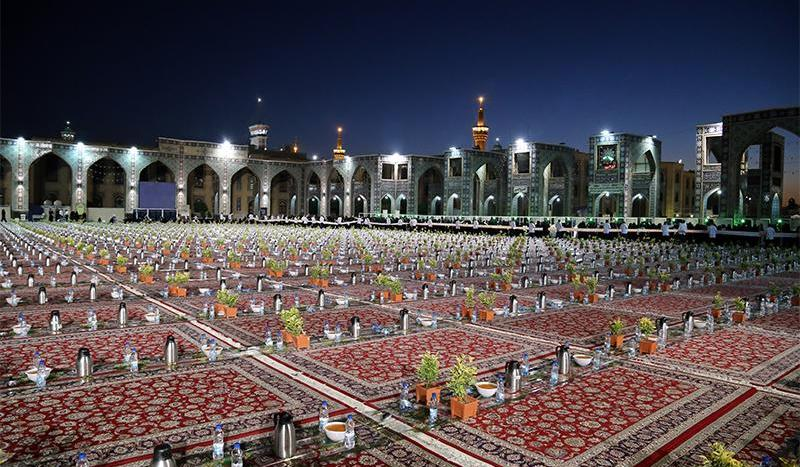
\includegraphics[width=0.65\linewidth]{images/nature_images/irs.jpg}
    \caption{A communal gathering}
    \end{center}
\end{figure}
The size of image is set here relative to line width  but you can use  \verb|\columnsep|, \verb|\textwidth|, \verb|\textheight|, \verb|\paperheight| etc..
\end{document}
\end{lstlisting}





%%%%%%%%%%%%%%%%%%%%%%%%%%%%%%%%%%%%%%%%%%%%%%%%%%%%%%%%%%%%%%%%%%
%                    NEW PAGE                                    %
%                     Images r                                   %
%                                                                %
%%%%%%%%%%%%%%%%%%%%%%%%%%%%%%%%%%%%%%%%%%%%%%%%%%%%%%%%%%%%%%%%%%
\newpage
\begin{tightcenter}
{\Huge \textbf{Images}}
\end{tightcenter}

 
By default latex will look for image file first in folder containing ``.tex'' file. You can use `relative path' such as \verb|images/image.jpg| or `absolute path' like \verb|C:\path\to\image.jpg| to the file.

\begin{figure}%[H]
    \begin{center}
    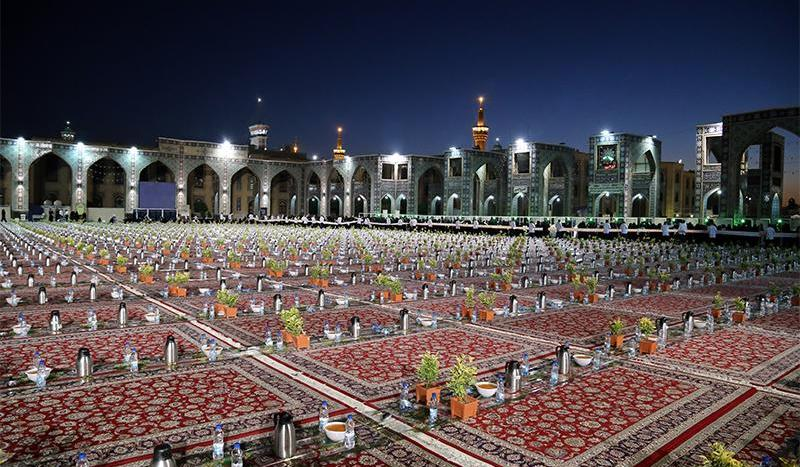
\includegraphics[width=0.65\linewidth]{images/nature_images/irs.jpg}
    \caption{A communal gathering}
    \end{center}
\end{figure}

The size of image is set here relative to line width but you can use  \verb|\columnsep|, \verb|\textwidth|, \verb|\textheight|, \verb|\paperheight| etc.


%%%%%%%%%%%%%%%%%%%%%%%%%%%%%%%%%%%%%%%%%%%%%%%%%%%%%%%%%%%%%%%%%%
%                    NEW PAGE                                    %
%                     Images 2c                                   %
%                                                                %
%%%%%%%%%%%%%%%%%%%%%%%%%%%%%%%%%%%%%%%%%%%%%%%%%%%%%%%%%%%%%%%%%%
\newpage
\begin{tightcenter}
{\Huge \textbf{Images}}
\end{tightcenter}





\begin{lstlisting}
\documentclass[10pt]{article}
\usepackage{graphicx}
\usepackage{float}
\begin{document} 
By default latex will place image wherever it deems proper but to put it where we want, use \verb|\usepackage{float}| and put \verb|[H]| to place it exactly where you wrote code for it. You can pass parameter \verb|t| or \verb|b| to place the image at top or bottom of page respectively.

\begin{figure}[H]
    \begin{center}
    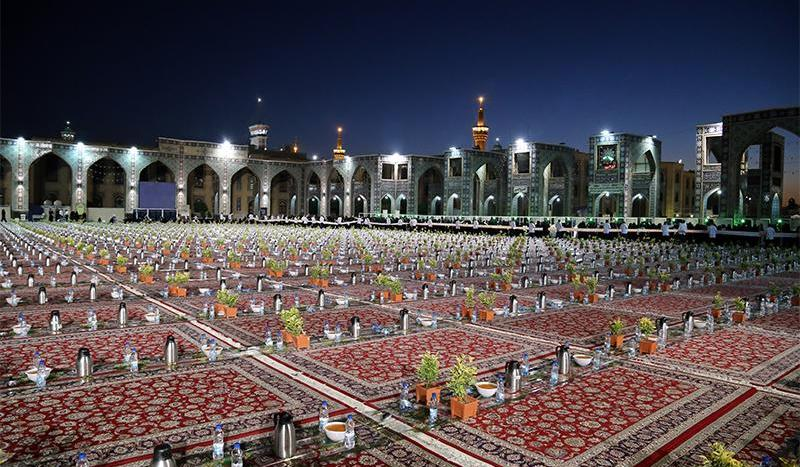
\includegraphics[width=4cm, height=2cm, angle=45]{images/nature_images/irs.jpg}
    \caption{A communal gathering}
    \end{center}
\end{figure}
\end{document}
\end{lstlisting}




%%%%%%%%%%%%%%%%%%%%%%%%%%%%%%%%%%%%%%%%%%%%%%%%%%%%%%%%%%%%%%%%%%
%                    NEW PAGE                                    %
%                     Images 2r                                   %
%                                                                %
%%%%%%%%%%%%%%%%%%%%%%%%%%%%%%%%%%%%%%%%%%%%%%%%%%%%%%%%%%%%%%%%%%
\newpage
\begin{tightcenter}
{\Huge \textbf{Images}}
\end{tightcenter}




By default latex will place image wherever it deems proper but to put it where we want, use \verb|\usepackage{float}| and put \verb|[H]| to place it exactly where you wrote code for it. You can pass parameter \verb|t| or \verb|b| to place the image at top or bottom of page respectively.

\begin{figure}[H]
    \begin{center}
    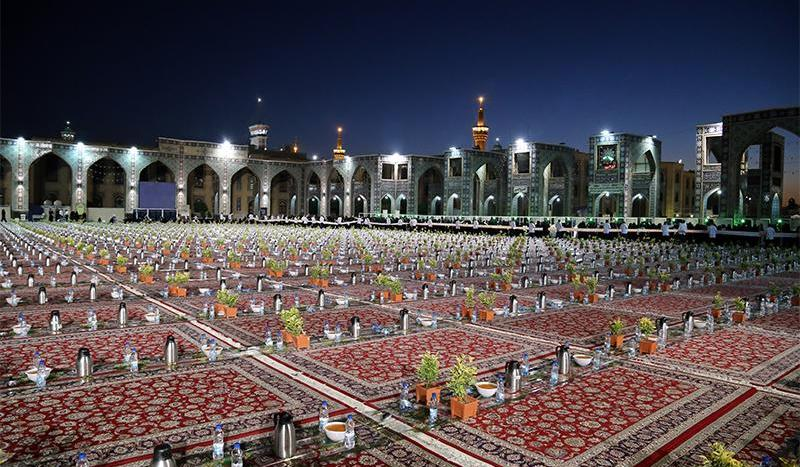
\includegraphics[width=4cm, height=2cm, angle=45]{images/nature_images/irs.jpg}
    \caption{A communal gathering}
    \end{center}
\end{figure}



%%%%%%%%%%%%%%%%%%%%%%%%%%%%%%%%%%%%%%%%%%%%%%%%%%%%%%%%%%%%%%%%%%
%                    NEW PAGE                                    %
%                     Images 3c                                   %
%                                                                %
%%%%%%%%%%%%%%%%%%%%%%%%%%%%%%%%%%%%%%%%%%%%%%%%%%%%%%%%%%%%%%%%%%
\newpage
\begin{tightcenter}
{\Huge \textbf{Images}}
\end{tightcenter}


\begin{lstlisting}
\documentclass[10pt]{article}
\usepackage{graphicx}
\usepackage{wrapfig}
\usepackage{float}
\newcommand{\nopar}{{\parfillskip=0pt \par}}
\usepackage{lipsum}
\begin{document} 
You can also wrap the figure around text by using \verb|\usepackage{wrapfig}| and placing your image inside \textit{wrapfigure} environment.  \nopar

\begin{wrapfigure}[11]{r}{4cm}
\centering
    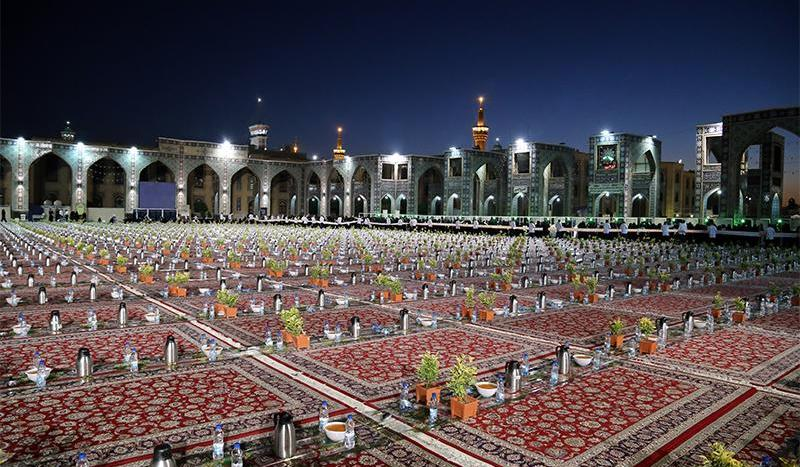
\includegraphics[scale=0.1, angle=45]{images/nature_images/irs.jpg}  
\end{wrapfigure}

\noindent
The first argument `r' puts it on right side and second argument defines container for the figure. 
This is some text without any meaning.This is some text without any meaning.This is some text without any meaning. This is some text without any meaning.This is some text without any meaning.This is some text without any meaning.This is some text without any meaning. \lipsum[1]
\end{lstlisting}





%%%%%%%%%%%%%%%%%%%%%%%%%%%%%%%%%%%%%%%%%%%%%%%%%%%%%%%%%%%%%%%%%%
%                    NEW PAGE                                    %
%                     Images 3r                                   %
%                                                                %
%%%%%%%%%%%%%%%%%%%%%%%%%%%%%%%%%%%%%%%%%%%%%%%%%%%%%%%%%%%%%%%%%%
\newpage
\begin{tightcenter}
{\Huge \textbf{Images}}
\end{tightcenter}



You can also wrap the figure around text by using \verb|\usepackage{wrapfig}| and placing your image inside \textit{wrapfigure} environment.  \nopar

\begin{wrapfigure}[11]{r}{4cm}
\centering
    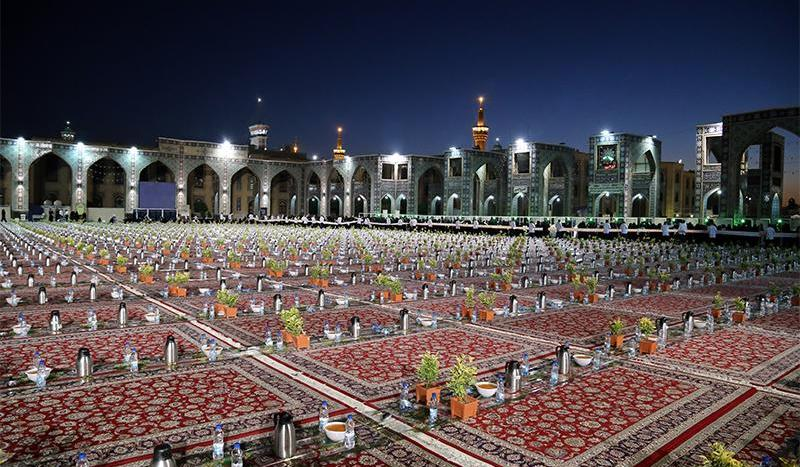
\includegraphics[scale=0.1, angle=45]{images/nature_images/irs.jpg}  
\end{wrapfigure}

\noindent
The first argument `r' puts it on right side and second argument defines container for the figure. 
This is some text without any meaning.This is some text without any meaning.This is some text without any meaning. This is some text without any meaning.This is some text without any meaning.This is some text without any meaning.This is some text without any meaning. \lipsum[1]





%%%%%%%%%%%%%%%%%%%%%%%%%%%%%%%%%%%%%%%%%%%%%%%%%%%%%%%%%%%%%%%%%%
%                    NEW PAGE                                    %
%                     Images 4c                                   %
%                                                                %
%%%%%%%%%%%%%%%%%%%%%%%%%%%%%%%%%%%%%%%%%%%%%%%%%%%%%%%%%%%%%%%%%%
\newpage
\begin{tightcenter}
{\Huge \textbf{Images}}
\end{tightcenter}


\begin{lstlisting}
\documentclass[10pt]{article}
\usepackage{graphicx}
\usepackage{float}
\begin{document} 
You can put two separate images side.  The argument \verb|!| means overriding internal latex parameters which define position of float image. \verb|h| means approximately at same position as appeared in code. 

\begin{figure}[!h]
    \centering
    \begin{minipage}{0.45\textwidth}
        \centering
        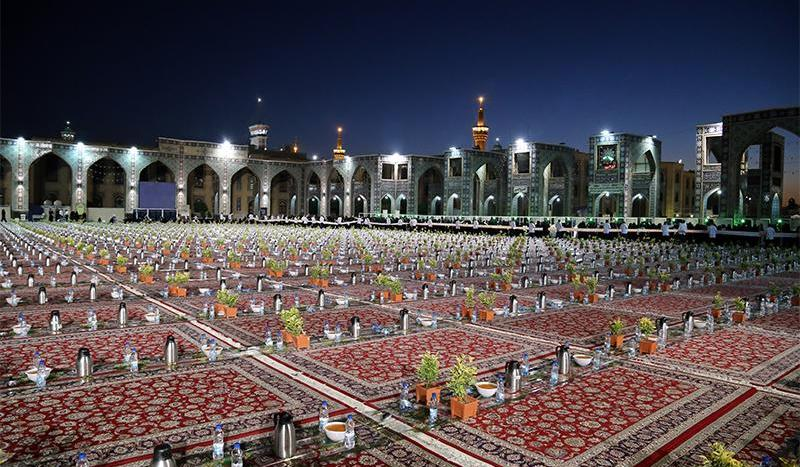
\includegraphics[width=0.9\textwidth]{images/nature_images/irs.jpg} % first figure itself
        \caption{an image}
    \end{minipage}\hfill
    \begin{minipage}{0.45\textwidth}
        \centering
        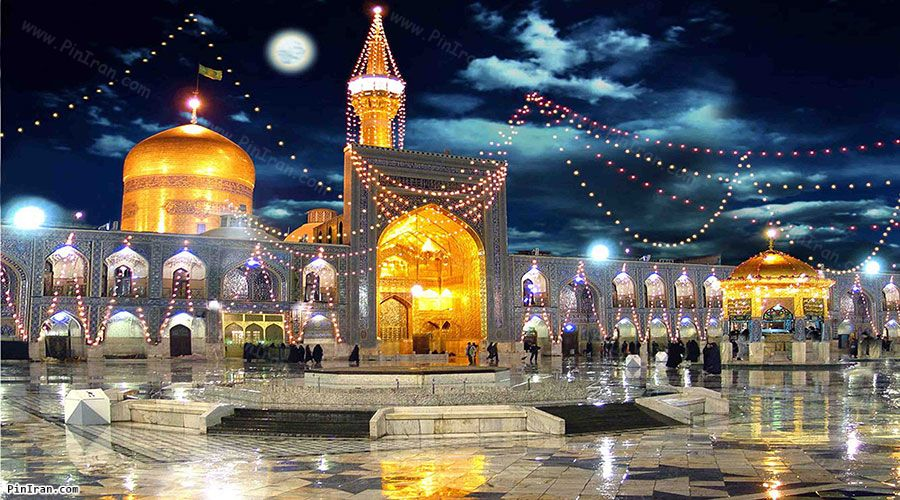
\includegraphics[width=1\textwidth]{images/nature_images/irs2.jpg} % second figure itself
        \caption{another image}
    \end{minipage}
\end{figure}
\verb|\hfill| fills the remaining horizontal space in line afterwards.
\end{document}
\end{lstlisting}





%%%%%%%%%%%%%%%%%%%%%%%%%%%%%%%%%%%%%%%%%%%%%%%%%%%%%%%%%%%%%%%%%%
%                    NEW PAGE                                    %
%                     Images 4r                                   %
%                                                                %
%%%%%%%%%%%%%%%%%%%%%%%%%%%%%%%%%%%%%%%%%%%%%%%%%%%%%%%%%%%%%%%%%%
\newpage
\begin{tightcenter}
{\Huge \textbf{Images}}
\end{tightcenter}




You can put two separate images side.  The argument \verb|!| means overriding internal latex parameters which define position of float image. \verb|h| means approximately at same position as appeared in code. 

\begin{figure}[!h]
    \centering
    \begin{minipage}{0.45\textwidth}
        \centering
        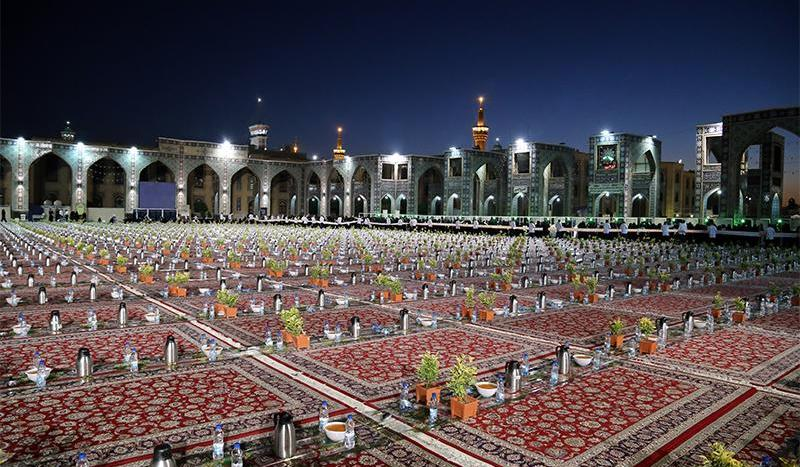
\includegraphics[width=0.9\textwidth]{images/nature_images/irs.jpg} % first figure itself
        \caption{an image}
    \end{minipage}\hfill
    \begin{minipage}{0.45\textwidth}
        \centering
        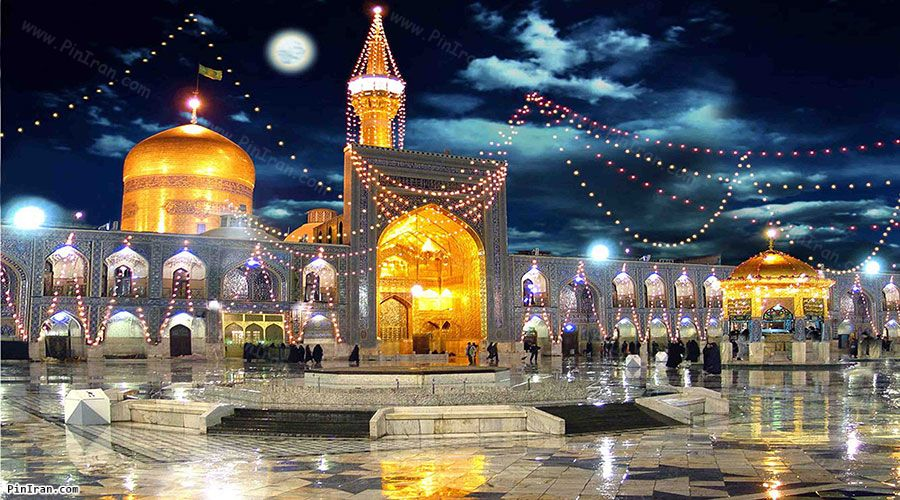
\includegraphics[width=1\textwidth]{images/nature_images/irs2.jpg} % second figure itself
        \caption{another image}
    \end{minipage}
\end{figure}
\verb|\hfill| fills the remaining horizontal space in line afterwards.







%%%%%%%%%%%%%%%%%%%%%%%%%%%%%%%%%%%%%%%%%%%%%%%%%%%%%%%%%%%%%%%%%%
%                    NEW PAGE                                    %
%                     Tables c                                   %
%                                                                %
%%%%%%%%%%%%%%%%%%%%%%%%%%%%%%%%%%%%%%%%%%%%%%%%%%%%%%%%%%%%%%%%%%
\newpage
\begin{tightcenter}
{\Huge \textbf{Tables}}
\end{tightcenter}





\begin{lstlisting}
\documentclass[10pt]{article}
\begin{document} 
You can write a table within \textit{tabular} environment. $\vert$ defines the vertical line in columns. Within table use ampersand \verb|&| to separate different entries in columns. Number of ``c" tells number of columns and the letter ``c" represents that text will be centered in cells. Use ``r" or ``l" for right or left justified text.
\begin{center}
 \begin{tabular}{||c c c c||} 
 \hline
 Book Name & Writer & Year Published & comments \\ %[0.5ex] 
 \hline\hline
Our Economy & Baqir al sadr  & 1960 &  about economy \\
\hline
Our Philosophy & Baqir al sadr  & 1959 &  about philosophy \\
\hline 
The Source Of Rights & Taqi Misbah Yazdi &  & \\
\hline
Causality and Freedom & Mohsen Araki & here & \\
\hline
Eternity of Man & & \  & \\
\hline
Perfect Man &   Murtadha Mutahhari & 1975  & \\
\hline
\end{tabular}
\end{center}
\end{document}
\end{lstlisting}






%%%%%%%%%%%%%%%%%%%%%%%%%%%%%%%%%%%%%%%%%%%%%%%%%%%%%%%%%%%%%%%%%%
%                    NEW PAGE                                    %
%                     Tables r                                   %
%                                                                %
%%%%%%%%%%%%%%%%%%%%%%%%%%%%%%%%%%%%%%%%%%%%%%%%%%%%%%%%%%%%%%%%%%
\newpage
\begin{tightcenter}
{\Huge \textbf{Tables}}
\end{tightcenter}


You can write a table within \textit{tabular} environment. $\vert$ defines the vertical line in columns. Within table use ampersand \verb|&| to separate different entries in columns. Number of ``c" tells number of columns and the letter ``c" represents that text will be centered in cells. Use ``r" or ``l" for right or left justified text.
\begin{table}[H]
\begin{center}
\caption{A table}
\label{tab:mytable1}
 \begin{tabular}{||c c c c||} 
 \hline
 Book Name & Writer & Year Published & comments \\ %[0.5ex] 
 \hline\hline
Our Economy & Baqir al sadr  & 1960 &  about economy \\
\hline
Our Philosophy & Baqir al sadr  & 1959 &  about philosophy \\
\hline 
The Source Of Rights & Taqi Misbah Yazdi &  & \\
\hline
Causality and Freedom & Mohsen Araki & here & \\
\hline
Eternity of Man & & \  & \\
\hline
Perfect Man &   Murtadha Mutahhari & 1975  & \\
\hline
\end{tabular}
\end{center}
\end{table}





%%%%%%%%%%%%%%%%%%%%%%%%%%%%%%%%%%%%%%%%%%%%%%%%%%%%%%%%%%%%%%%%%%
%                    NEW PAGE                                    %
%                     Tables 2c                                   %
%                                                                %
%%%%%%%%%%%%%%%%%%%%%%%%%%%%%%%%%%%%%%%%%%%%%%%%%%%%%%%%%%%%%%%%%%
\newpage
\begin{tightcenter}
{\Huge \textbf{Tables}}
\end{tightcenter}




\begin{lstlisting}
\documentclass[10pt]{article}
\usepackage{multirow}
\begin{document} 
You can fix the cell widths. One `pt' is equal to \(\sim\)0.35mm. The text alignment options are `\texttt{p}' for top, `\texttt{m}' for middle and `\texttt{b}' for bottom of cell. You can use \verb|\multirow{no of cells}{width}{text}| and \verb|\multicolumn{}{}{}| to combine rows and columns.
\begin{table}[h]
\centering
\caption{My caption}
\label{my-label}
\begin{tabular}{|l|l|l|l|l|}
\hline
\multirow{2}{*}{\textbf{Writer}} & \multirow{2}{*}{\textbf{Book name}} & \multirow{2}{*}{Editions} & \multicolumn{2}{l|}{Availability} \\ \cline{4-5} 
  &  &  & online & free \\
 \hline
\multirow{4}{*}{Nietsche} & \multirow{4}{*}{Zarathustra} &  & & \\
\cline{3-5} 
 &  & c4.5 &  & \\ \cline{3-5} 
 &  &   & &  \\ \cline{3-5} 
 &  &   & &  \\ \hline
\multirow{4}{*}{Shakespear} & \multirow{4}{*}{Othello} &   & & \\
\cline{3-5} 
 &  & c4.5 & & \\ \cline{3-5} 
 &  &   & & \\ \cline{3-5} 
 &  &   &  & \\ \hline
\multirow{4}{*}{Karl Marx} & \multirow{4}{*}{Das Kapital} &   && \\
\cline{3-5} 
 &  & c4.5 & &  \\ \cline{3-5} 
 &  &   & &  \\ \cline{3-5} 
 &  &   & &  \\ \hline
\multirow{4}{*}{Frantz Fannon} & \multirow{4}{*}{The wretched of the earth} &   & & \\
\cline{3-5} 
 &  & c4.5 & &  \\ \cline{3-5} 
 &  &   &  & \\ \cline{3-5} 
 &  &   & & \\ \hline
\end{tabular}
\end{table}
\verb|\cline| command makes a horizontal line only below certain columns defined.
\end{document}
\end{lstlisting}





%%%%%%%%%%%%%%%%%%%%%%%%%%%%%%%%%%%%%%%%%%%%%%%%%%%%%%%%%%%%%%%%%%
%                    NEW PAGE                                    %
%                     Tables 2c                                   %
%                                                                %
%%%%%%%%%%%%%%%%%%%%%%%%%%%%%%%%%%%%%%%%%%%%%%%%%%%%%%%%%%%%%%%%%%
\newpage
\begin{tightcenter}
{\Huge \textbf{Tables}}
\end{tightcenter}




You can fix the cell widths. One `pt' is equal to \(\sim\)0.35mm. The text alignment options are `\texttt{p}' for top, `\texttt{m}' for middle and `\texttt{b}' for bottom of cell. You can use \verb|\multirow{no of cells}{width}{text}| and \verb|\multicolumn{}{}{}| to combine rows and columns.
\begin{table}[H]
\centering
\caption{My caption}
\label{my-label}
\begin{tabular}{|l|l|l|l|l|}
\hline
\multirow{2}{*}{\textbf{Writer}} & \multirow{2}{*}{\textbf{Book name}} & \multirow{2}{*}{Editions} & \multicolumn{2}{l|}{Availability} \\ \cline{4-5} 
  &  &  & online & free \\
 \hline
\multirow{4}{*}{Nietsche} & \multirow{4}{*}{Zarathustra} &  & & \\
\cline{3-5} 
 &  & c4.5 &  & \\ \cline{3-5} 
 &  &   & &  \\ \cline{3-5} 
 &  &   & &  \\ \hline
\multirow{4}{*}{Shakespear} & \multirow{4}{*}{Othello} &   & & \\
\cline{3-5} 
 &  & c4.5 & & \\ \cline{3-5} 
 &  &   & & \\ \cline{3-5} 
 &  &   &  & \\ \hline
\multirow{4}{*}{Frantz Fannon} & \multirow{4}{*}{The wretched of the earth} &   & & \\
\cline{3-5} 
 &  & c4.5 & &  \\ \cline{3-5} 
 &  &   &  & \\ \cline{3-5} 
 &  &   & & \\ \hline
\end{tabular}
\end{table}
\verb|\cline| command makes a horizontal line only below certain columns defined.






%%%%%%%%%%%%%%%%%%%%%%%%%%%%%%%%%%%%%%%%%%%%%%%%%%%%%%%%%%%%%%%%%%
%                    NEW PAGE                                    %
%                     Tables 3c                                   %
%                                                                %
%%%%%%%%%%%%%%%%%%%%%%%%%%%%%%%%%%%%%%%%%%%%%%%%%%%%%%%%%%%%%%%%%%
\newpage
\begin{tightcenter}
{\Huge \textbf{Tables}}
\end{tightcenter}

\setlength{\arrayrulewidth}{1mm}  % lines in columns
\renewcommand{\arraystretch}{1.5} % height of each row

For multiplage table use the environment \texttt{longtable} provided by package \texttt{longtable}


\begin{center}
\label{tab:mylongtable}
 \begin{longtable}[ht]{|p{3cm}|p{3cm}|p{3cm}|p{3cm}|} 
 \hline
 Book Name & Writer & Year Published & comments \\ %[0.5ex] 
 \hline
Our Economy & Baqir al sadr  & 1960 &  about economy \\
\hline
Our Philosophy & Baqir al sadr  & 1959 &  about philosophy \\
\hline 
The Source Of Rights & Taqi Misbah Yazdi &  & \\
\hline
\rowcolor{lightgray}Causality and Freedom & Mohsen Araki & here & \\
\hline
Eternity of Man & & \  & \\
\hline
Perfect Man &   Murtadha Mutahhari & 1975  & \\
\hline
 Book Name & Writer & Year Published & comments \\ %[0.5ex] 
 \hline
Our Economy & Baqir al sadr  & 1960 &  about economy \\
\hline
Our Philosophy & Baqir al sadr  & 1959 &  \cellcolor{blue} about philosophy \\
\hline 
The Source Of Rights & Taqi Misbah Yazdi &  & \\
\hline


\end{longtable}
\end{center}





%%%%%%%%%%%%%%%%%%%%%%%%%%%%%%%%%%%%%%%%%%%%%%%%%%%%%%%%%%%%%%%%%%
%                    NEW PAGE                                    %
%            Hypertext and hyper-reference                       %
%                                                                %
%%%%%%%%%%%%%%%%%%%%%%%%%%%%%%%%%%%%%%%%%%%%%%%%%%%%%%%%%%%%%%%%%%
\newpage
\begin{tightcenter}
{\Huge \textbf{Hypertext and hyper-reference}}
\end{tightcenter}

\setlength{\arrayrulewidth}{0.2mm}  % lines in columns
\renewcommand{\arraystretch}{0.8} % height of each row

\begin{table}[H]
\begin{center}
\caption{A table}
\label{tab:mytable}
 \begin{tabular}{|c c c c|} 
 \hline
 Book Name & Writer & Year Published & comments \\ %[0.5ex] 
 \hline
Our Economy & Baqir al sadr  & 1960 &  about economy \\
\hline
\end{tabular}
\end{center}
\end{table}

\begin{figure}[H]
    \begin{center}
    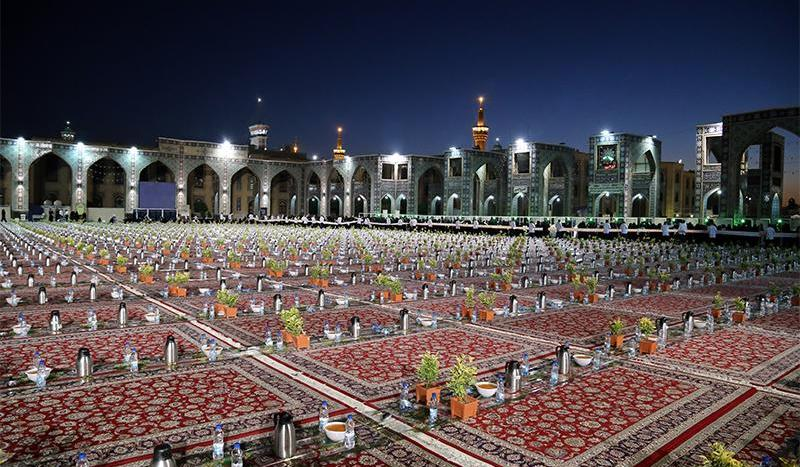
\includegraphics[width=0.25\linewidth]{images/nature_images/irs.jpg}
    \caption{A communal gathering}
    \label{fig:myfigure}
    \end{center}
\end{figure}
\begin{align}  \label{eq:myeq}
\begin{split}
S_s &=\frac{S}{b}
\end{split}					
\end{align}

Table \ref{tab:mytable1} and figure \ref{fig:myfigure} and equation \href{eq:myeq}{ \ref{eq:myeq}} can be hyper-referenced as shown in this \href{https://www.overleaf.com/learn/latex/Hyperlinks}{link}. 




%%%%%%%%%%%%%%%%%%%%%%%%%%%%%%%%%%%%%%%%%%%%%%%%%%%%%%%%%%%%%%%%%%
%                    NEW PAGE                                    %
%            Hypertext and hyper-reference                       %
%                                                                %
%%%%%%%%%%%%%%%%%%%%%%%%%%%%%%%%%%%%%%%%%%%%%%%%%%%%%%%%%%%%%%%%%%
\newpage
\begin{tightcenter}
{\Huge \textbf{Hypertext and hyper-reference}}
\end{tightcenter}

\begin{lstlisting}
\documentclass[10pt]{article}
\usepackage{graphicx, float, amsmath}
\usepackage[colorlinks]{hyperref}
\hypersetup{  colorlinks = true,  linkcolor  = black,  citecolor= blue}
\begin{document} 
\begin{table}[H]
\begin{center} \caption{A table} \label{tab:mytable1}
 \begin{tabular}{|c c c c|} 
 \hline
 Book Name & Writer & Year Published & comments \\ %[0.5ex] 
 \hline
Our Economy & Baqir al sadr  & 1960 &  about economy \\
\hline
\end{tabular} \end{center} \end{table} 
\begin{figure}[H]
    \begin{center}
    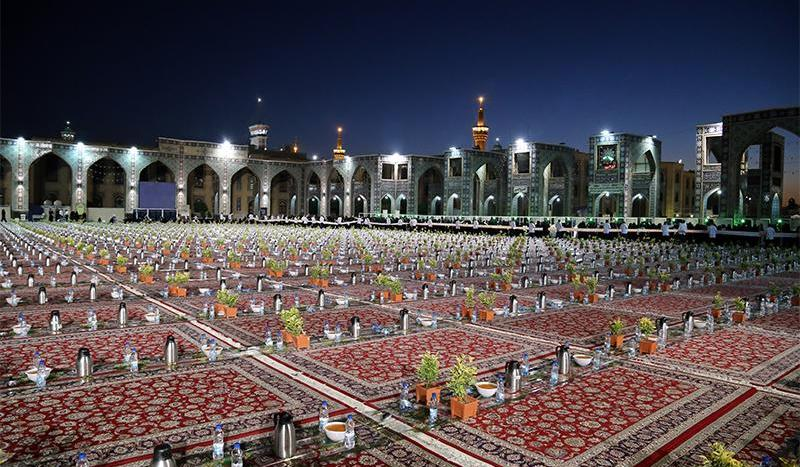
\includegraphics[width=0.25\linewidth]{images/nature_images/irs.jpg}
    \caption{A communal gathering}
    \label{fig:myfigure}
    \end{center} \end{figure}
\begin{align}  \label{eq:myeq}
\begin{split}
S_s &=\frac{S}{b}
\end{split}	\end{align}
Table \ref{tab:mytable1} and figure \ref{fig:myfigure} and equation \href{eq:myeq}{ \ref{eq:myeq}} can be hyper-referenced as shown in this \href{https://www.overleaf.com/learn/latex/Hyperlinks}{link}. 
\end{document}
\end{lstlisting}




%%%%%%%%%%%%%%%%%%%%%%%%%%%%%%%%%%%%%%%%%%%%%%%%%%%%%%%%%%%%%%%%%%
%                    NEW PAGE                                    %
%                  Bibliography                                  %
%                                                                %
%%%%%%%%%%%%%%%%%%%%%%%%%%%%%%%%%%%%%%%%%%%%%%%%%%%%%%%%%%%%%%%%%%
\newpage
\begin{tightcenter}
{\Huge \textbf{Bibliography}}
\end{tightcenter}

In order to cite a work, put its reference in a file `bib\_file.bib'. The reference format for a book is as below. 
\begin{lstlisting}
@book{Gerya2010,
author    = "Gerya T V.",
title     = "Introduction to Numerical Geodynamic Modeling",
publisher = "Cambridge University Press",
year      = "2010",
}
\end{lstlisting}
One can download the whole reference for a work from internet. Put all of your references in the file with extension `.bib'. Then in the `.tex' file you can cite the work of \cite{Gerya:2010}. In order to place references in your document, use following two commands

\begin{lstlisting}
\bibliographystyle{cell}
\bibliography{bib_file}
\end{lstlisting}

Don't forget to put \verb|\usepackage[square]{natbib}| in preamble.





\bibliographystyle{cell}
\bibliography{bib_file}



%%%%%%%%%%%%%%%%%%%%%%%%%%%%%%%%%%%%%%%%%%%%%%%%%%%%%%%%%%%%%%%%%%
%                    NEW PAGE                                    %
%            Create your own environment                         %
%                                                                %
%%%%%%%%%%%%%%%%%%%%%%%%%%%%%%%%%%%%%%%%%%%%%%%%%%%%%%%%%%%%%%%%%%
\newpage
\begin{tightcenter}
{\Huge \textbf{Create your own environment}}
\end{tightcenter}


\begin{lstlisting}
\documentclass[10pt]{article}
\usepackage[linewidth=2pt]{mdframed}
\newenvironment{tightcenter}{%
  \setlength\topsep{0pt}
  \setlength\parskip{0pt}
  \begin{mdframed}
  \begin{center}
}{%
  \end{center}
  \vspace{20pt}  % leave some space below text
  \end{mdframed}
}
\begin{document}
\begin{tightcenter}
This is inside `tightcenter' environment.
\end{tightcenter}
\end{document}
\end{lstlisting}

\begin{mdframed}
\begin{tightcenter}
This is inside `tightcenter' environment. 
\end{tightcenter}
\end{mdframed}

Instead of writing four commands we combine 4 commands into one and call the new command \textit{tightcenter} and this new command executes all 4 commands.



%%%%%%%%%%%%%%%%%%%%%%%%%%%%%%%%%%%%%%%%%%%%%%%%%%%%%%%%%%%%%%%%%%
%                    NEW PAGE                                    %
%            Create your own environment                         %
%                                                                %
%%%%%%%%%%%%%%%%%%%%%%%%%%%%%%%%%%%%%%%%%%%%%%%%%%%%%%%%%%%%%%%%%%
\newpage
\begin{tightcenter}
{\Huge \textbf{Create your own environment}}
\end{tightcenter}


\begin{lstlisting}
\documentclass[10pt]{article}
\usepackage[linewidth=2pt]{mdframed}
\newenvironment{tightcenter}{%
  \setlength\topsep{0pt}
  \setlength\parskip{0pt}
  \begin{mdframed}
  \begin{center}
}{%
  \end{center}
  \end{mdframed}
  \vspace{20pt}  % leave some space below text
}
\begin{document}
\begin{tightcenter}
Can you identify the change between this and previous environment?.
\end{tightcenter}
\end{document}
\end{lstlisting}

\newenvironment{Ntightcenter}{%
  \setlength\topsep{0pt}
  \setlength\parskip{0pt}
  \begin{mdframed}
  \begin{center}
}{%
  \end{center}
  \end{mdframed}
  \vspace{20pt}  % leave some space below text
}


\begin{Ntightcenter}
Can you identify the change between this and previous environment?.
\end{Ntightcenter}






%%%%%%%%%%%%%%%%%%%%%%%%%%%%%%%%%%%%%%%%%%%%%%%%%%%%%%%%%%%%%%%%%%
%                    NEW PAGE                                    %
%                       Track changes                            %
%                                                                %
%%%%%%%%%%%%%%%%%%%%%%%%%%%%%%%%%%%%%%%%%%%%%%%%%%%%%%%%%%%%%%%%%%
\newpage
\begin{tightcenter}
{\Huge \textbf{Track changes}}
\end{tightcenter}

\begin{abstract} \noindent The intention of this text is to demonstrate the use of \texttt{trackchanges.sty}. The package defines five editing commands:
\begin{itemize}
  \item \begin{verbatim}\note[initials]{note text}\end{verbatim}
  \item \begin{verbatim}\annote[initials]{note text}\end{verbatim}
  \item \begin{verbatim}\add[initials]{additional text}\end{verbatim}
  \item \begin{verbatim}\remove[initials]{removed text}\end{verbatim}
  \item \begin{verbatim}\change[initials]{original text}{new text}\end{verbatim}
\end{itemize}
\end{abstract}
\section*{Introduction} 
The purpose of this document is to show how to do some \add[FS]{complex} changes in document in collaborative writing as done in \change[PS]{Microsoft Office}{OpenOffice.org}. Overleaf now provides more robust way of tracking changes in latex source code\note[FS]{Should I describe the methodology of overleaf}. But it is only possible when you have internet \remove[PS]{connection}.
You can use any source control package like \emph{git} to achieve same thing \annote[PS]{though}{what about PDF? The changes can be seen in PDF as well? ...}.



%%%%%%%%%%%%%%%%%%%%%%%%%%%%%%%%%%%%%%%%%%%%%%%%%%%%%%%%%%%%%%%%%%
%                    NEW PAGE                                    %
%                   Track changes                                %
%                                                                %
%%%%%%%%%%%%%%%%%%%%%%%%%%%%%%%%%%%%%%%%%%%%%%%%%%%%%%%%%%%%%%%%%%
\newpage
\begin{tightcenter}
{\Huge \textbf{Track changes}}
\end{tightcenter}


\begin{lstlisting}
\documentclass[a4paper,10pt]{article}
\usepackage{url}
\usepackage{trackchanges}
\renewcommand{\initialsOne}{FS}
\renewcommand{\initialsTwo}{PS}
\begin{document}
\begin{abstract} \noindent The intention of this text is to demonstrate the use of \texttt{trackchanges.sty}. The package defines five editing commands:
\begin{itemize}
  \item \begin{verbatim}\note[initials]{note text}\end{verbatim}
  \item \begin{verbatim}\annote[initials]{note text}\end{verbatim}
  \item \begin{verbatim}\add[initials]{additional text}\end{verbatim}
  \item \begin{verbatim}\remove[initials]{removed text}\end{verbatim}
  \item \begin{verbatim}\change[initials]{original text}{new text}\end{verbatim}
\end{itemize}
\end{abstract}
\section*{Introduction} 
The purpose of this document is to show how to do some \add[FS]{complex} changes in document in collaborative writing as done in \change[PS]{Microsoft Office}{OpenOffice.org}. Overleaf now provides more robust way of tracking changes in latex source code\note[FS]{Should I describe the methodology of overleaf}. But it is only possible when you have internet \remove[PS]{connection}.
You can use any source control package like \emph{git} to achieve same thing \annote[PS]{though}{what about PDF? The changes can be seen in PDF as well? ...}.
\end{document}
\end{lstlisting}




%%%%%%%%%%%%%%%%%%%%%%%%%%%%%%%%%%%%%%%%%%%%%%%%%%%%%%%%%%%%%%%%%%
%                    NEW PAGE                                    %
%                   Generate Tables                              %
%                                                                %
%%%%%%%%%%%%%%%%%%%%%%%%%%%%%%%%%%%%%%%%%%%%%%%%%%%%%%%%%%%%%%%%%%
\newpage
\begin{tightcenter}
{\Huge \textbf{Generate Tables}}
\end{tightcenter}

\begin{table}[h!]
  \begin{center}
    \caption{table from .csv file}
    \label{tablex}
    \pgfplotstabletypeset[
      multicolumn names, % allows to have multicolumn names
      col sep=comma, % the seperator in our .csv file
      display columns/0/.style={
		column name=$Value 1$, % name of first column
		column type={S},string type},  % use siunitx for formatting
      display columns/1/.style={
		column name=$Value 2$,
		column type={S},string type},
      display columns/2/.style={
		column name=$Value 3$,
		column type={S},string type},
      every head row/.style={
		before row={\toprule}, % have a rule at top
		after row={
			\si{\ampere} & \si{\volt} & status\\ % the units seperated by &
			\midrule} % rule under units
			},
		every last row/.style={after row=\bottomrule}, % rule at bottom
    ]{table.csv} % filename/path to file
  \end{center}
\end{table}




%%%%%%%%%%%%%%%%%%%%%%%%%%%%%%%%%%%%%%%%%%%%%%%%%%%%%%%%%%%%%%%%%%
%                    NEW PAGE                                    %
%                   Generate Tables                              %
%                                                                %
%%%%%%%%%%%%%%%%%%%%%%%%%%%%%%%%%%%%%%%%%%%%%%%%%%%%%%%%%%%%%%%%%%
\newpage
\begin{tightcenter}
{\Huge \textbf{Generate Tables}}
\end{tightcenter}


\begin{lstlisting}
\documentclass{article}
\usepackage{booktabs} % For \toprule, \midrule and \bottomrule
\usepackage{siunitx} % Formats the units and values
\usepackage{pgfplotstable} % Generates table from .csv
\sisetup{  round-mode          = places, % Rounds numbers
  round-precision     = 2, % to 2 places
}
\begin{document}
\begin{table}[h!]   \begin{center}     \caption{table from .csv file}
    \pgfplotstabletypeset[
      multicolumn names, % allows to have multicolumn names
      col sep=comma, % the seperator in our .csv file
      display columns/0/.style={
		column name=$Value 1$, % name of first column
		column type={S},string type},  % use siunitx for formatting
      display columns/1/.style={
		column name=$Value 2$,
		column type={S},string type},
      display columns/2/.style={column name=$Value 3$,	column type={S},string type},
      every head row/.style={before row={\toprule}, % have a rule at top
		after row={
			\si{\ampere} & \si{\volt} & status\\ % the units seperated by &
			\midrule} % rule under units
			},
		every last row/.style={after row=\bottomrule}, % rule at bottom
    ]{table.csv} % filename/path to file
  \end{center} \end{table} \end{document}
\end{lstlisting}


\end{document}
%This document is part of the trackchanges sourceforge project and is published under GNU Public License version 2 or above
